\section{Rank-2 Systems}

\begin{frame}{Constructing Rank-2 Root Systems}
    In a 2-dimensional root space ($rank = 2$), we pick two roots $\alpha, \beta$ spanning $E$ and saturate the space by applying:
    \begin{enumerate}
        \item Weyl reflections $s_\alpha(\beta) = \beta - n_{\alpha\beta}\alpha$.
        \item The $\alpha$-string property (Thm 4.4.2): if $(\alpha, \beta) > 0$, then $\alpha - \beta \in \mathcal{R}$.
    \end{enumerate}

    \vspace{0.3cm}
    This purely geometric construction yields exactly 4 systems:

    \begin{figure}
        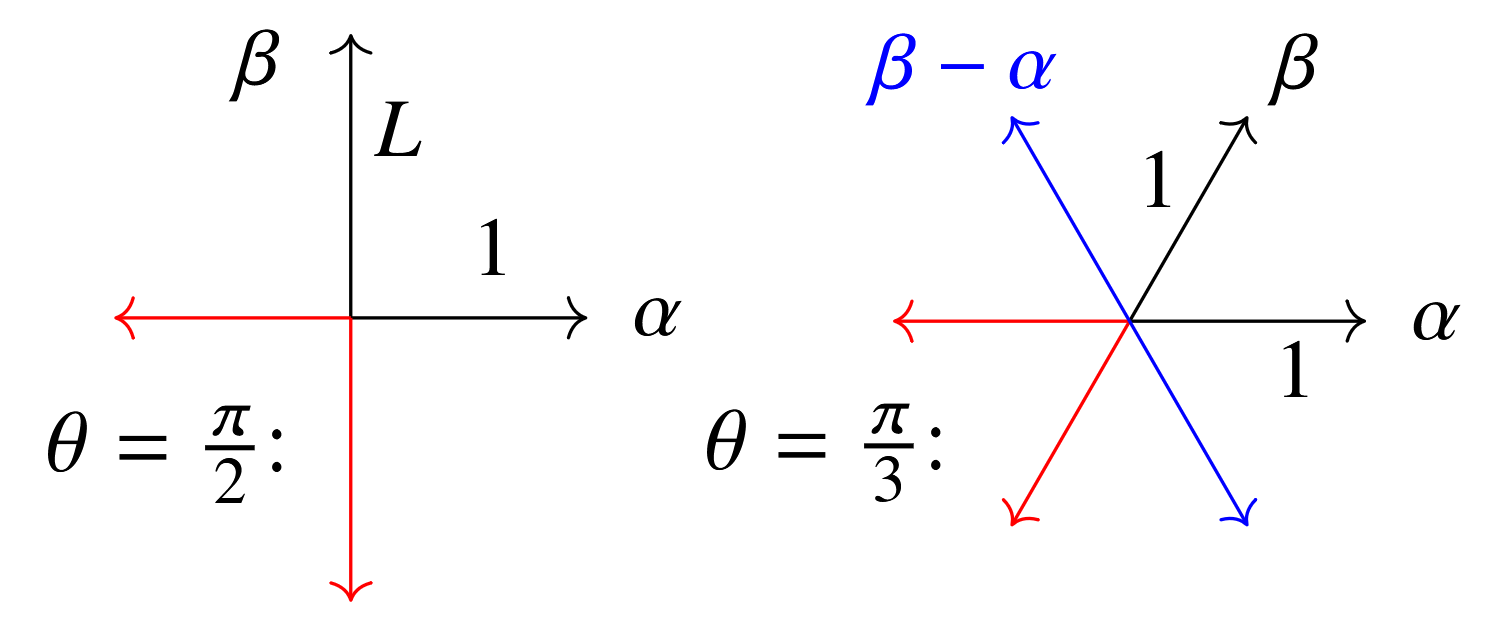
\includegraphics[width=0.7\textwidth]{img/A1-A2.png}
    \end{figure}

    % VOCAL CUE: Mostra alla lavagna A1+A1 (su2 x su2) e A2 (su3, sapore dei quark!).
\end{frame}

\begin{frame}{Rank-2 Root Systems: $B_2$ and $G_2$}
    For the remaining allowed angles, the reflection symmetries generate highly structured lattices:

    \begin{figure}
        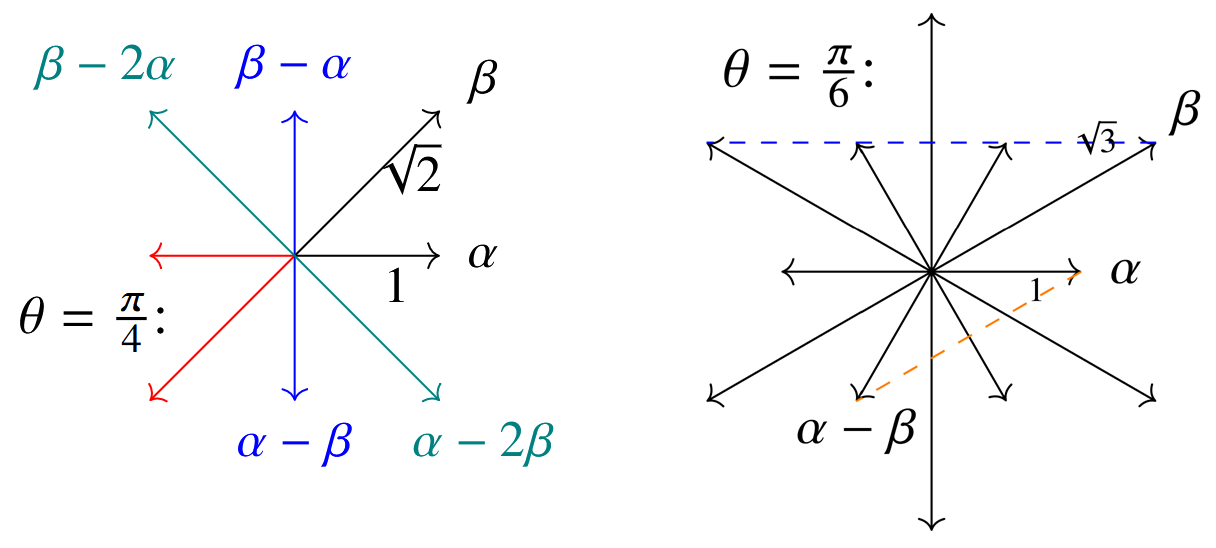
\includegraphics[width=0.7\textwidth]{img/B2-G2.png}
    \end{figure}

    % VOCAL CUE: B2 is isomorphic to so(5). G2 is exceptional, the first non-matrix Lie algebra!
    \vfill
    \hyperlink{backup_astring}{\beamerbutton{Theorem 4.4.2: Root Strings}}
\end{frame}